% Created 2015-10-23 Fri 15:33
\documentclass{scrartcl}
\usepackage[utf8]{inputenc}
\usepackage[T1]{fontenc}
\usepackage{fixltx2e}
\usepackage{graphicx}
\usepackage{longtable}
\usepackage{float}
\usepackage{wrapfig}
\usepackage{soul}
\usepackage{textcomp}
\usepackage{marvosym}
\usepackage{wasysym}
\usepackage{latexsym}
\usepackage{amssymb}
\usepackage{hyperref}
\tolerance=1000
\usepackage[margin=18mm]{geometry}
\usepackage{amsmath}
\usepackage{gensymb}
\usepackage{graphicx}
\usepackage{subfigure}
\usepackage{parskip}
\usepackage{standalone}
\usepackage{tikz,pgf,pgfplots}
\usetikzlibrary{decorations.pathmorphing,patterns}
\usetikzlibrary{arrows,snakes,backgrounds,patterns,matrix,shapes,fit,calc,shadows,plotmarks,decorations.markings,datavisualization,datavisualization.formats.functions,intersections,external}
\pgfplotsset{compat=1.9}
\newcommand*{\mexp}[1]{\ensuremath{\mathrm{e}^{#1}}}
\newcommand*{\laplace}[1]{\ensuremath{\mathcal{L} \{#1\}}}
\newcommand*{\laplaceinv}[1]{\ensuremath{\mathcal{L}^{-1} \{#1\}}}
\newcommand*{\realpart}[1]{\ensuremath{\operatorname{Re}(#1)}}
\newcommand*{\impart}[1]{\ensuremath{\operatorname{Im}(#1)}}
\newcommand*{\vsp}[1]{\rule{0pt}{#1}}
\newcommand*{\tderiv}[1]{\ensuremath{\frac{d^{#1}}{dt^{n}}}}
\newcommand*{\bbm}{\begin{bmatrix}}
\newcommand*{\ebm}{\end{bmatrix}}
\newcommand*{\obsmatrix}{\mathcal{O}}
\newcommand*{\contrmatrix}{\mathcal{C}}
\newcommand*{\cwh}{\ensuremath{\cos \omega h}}
\newcommand*{\swh}{\ensuremath{\sin \omega h}}
\newcommand*{\zethree}{\big(z - \mexp{-3h}\big)}
\providecommand{\alert}[1]{\textbf{#1}}

\title{Computerized control - preparation for partial exam 2}
\author{Kjartan Halvorsen}
\date{\today}
\hypersetup{
  pdfkeywords={},
  pdfsubject={},
  pdfcreator={Emacs Org-mode version 7.9.3f}}

\begin{document}

\maketitle



\section{Controller design}
\label{sec-1}


  A continous-time system is given by the transfer function
  \[ G(s) = \frac{1}{s}\left(\frac{-s+2}{s+2}\right).\]
  The system is to be controlled using error feedback
  \[ U(s) = F(s) \big(U_c(s) - Y(s) \big). \]

  \textbf{(a)} Determine the controller $F(s)$ so that the closed-loop system has the transfer function
  \[G_c(s) = \left(\frac{-s+2}{s+2}\right)\frac{1}{1+s/3}. \]
  Hint: Write $F(s)$ as a function of $G$ and $G_c$. 

  \textbf{(b)} Figure \ref{fig:nonminclosed} shows the Bode diagram of two different systems. Which of the graphs (solid or dashed lines) correspond to the closed-loop system?  OBS: only the phase curves differ. What is the band-width of the closed-loop system?
  \begin{figure}
  \begin{center}
  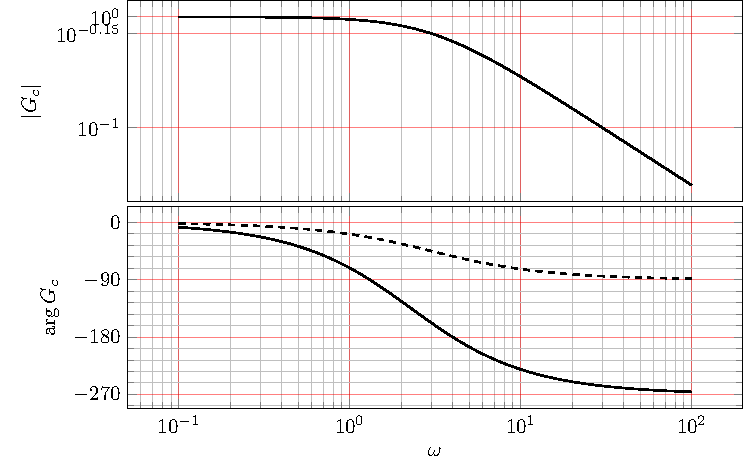
\includegraphics[width=0.8\linewidth]{bode-nonminphase}
  \end{center}
  \caption{Bode diagram of the closed-loop system. Which is the correct phase-curve?}
  \label{fig:nonminclosed}
  \end{figure}

  \textbf{(c)} Figure \ref{fig:nonminopen} shows the Bode diagram of the open-loop transfer function using the controller from exercise (a). What cross-over frequency and phase-marginal was achieved with the controller?
  \begin{figure}
  \begin{center}
  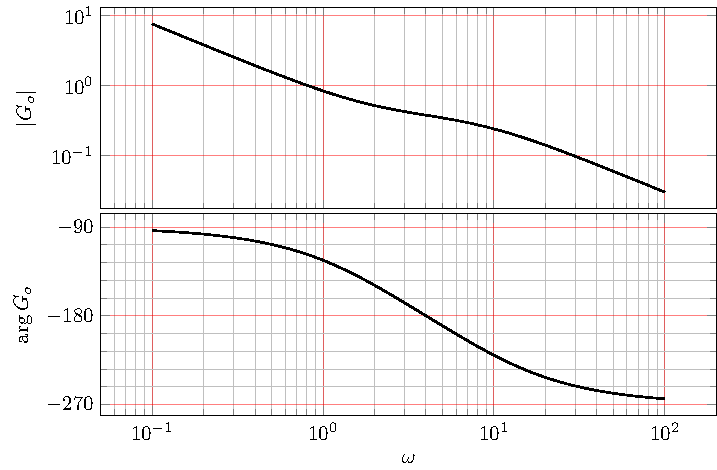
\includegraphics[width=0.8\linewidth]{bode-nonminopen}
  \end{center}
  \caption{Bode diagram of the open-loop system. What is the cross-over frequency and phase margin?}
  \label{fig:nonminopen}
  \end{figure}

  \textbf{(d)} Obtain a sampled controller using Tustin's approximation.
\section{PID tuning}
\label{sec-2}

  Figure \ref{fig:critical} shows the step-response from an experiment to find the ultimate gain and the ultimate period for the system in exercise 1.
  \begin{figure}
  \begin{center}
  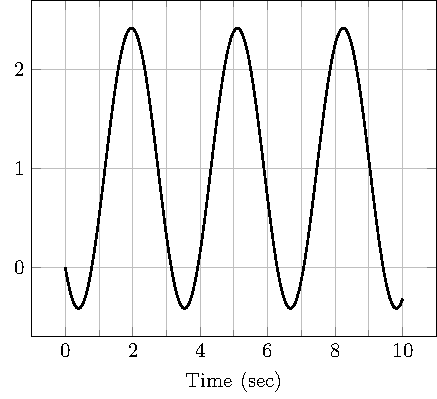
\includegraphics[width=0.5\linewidth]{bode-nonmincritical}
  \end{center}
  \caption{Step-response with ultimate gain. What is the ultimate period?}
  \label{fig:critical}
  \end{figure}

  \textbf{(a)} What is the ultimate period?

  \textbf{(b)} The gain is $K_u=2$. Write down the PID-controller obtained from the Ziegler-Nichols tuning method using the table 8.3 in Å\&W.

  \textbf{(c)} Figure \ref{fig:step} shows the step-responses of the closed-system obtained with the controller in exercise 1 (dashed) and with the controller using PID tuning (solid). How do they differ, and what does this say about the difference in phase margin and cross-over frequency? Why does the response with PID controller have a jump at $t=0$? Why do both responses start in the wrong direction (negative)?
  \begin{figure}
  \begin{center}
  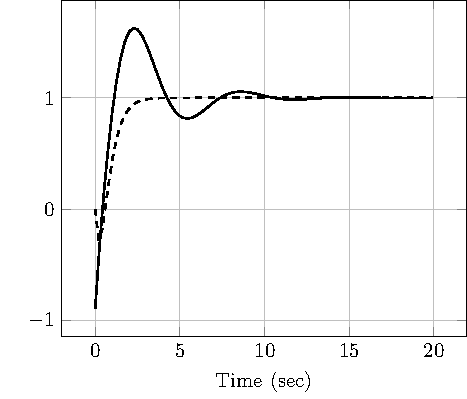
\includegraphics[width=0.5\linewidth]{bode-nonminstep}
  \end{center}
  \caption{Step-responses using the two controllers from exercise 1 and 2. What are the interesting differences?}
  \label{fig:step}
  \end{figure}

 
  \textbf{(d)} Obtain a sampled controller using backward difference (for all parts of the PID). 
  
\section{Solutions}
\label{sec-3}
\subsection{Controller design}
\label{sec-3-1}

   \textbf{(a)}
The close-loop system is given by
\[ G_c = \frac{GF}{1+GF}. \]
Solving this for $F$ gives
\begin{align*}
 F &= \frac{G_c}{G(1-G_c)} = \frac{ \left( \frac{-s+2}{s+2} \right) \frac{1}{1+s/3} } { \frac{-s+2}{s(s+2)}\left(1 - \left( \frac{-s+2}{s+2} \right) \frac{1}{1+s/3}\right)}\\
   &=  \frac{s}{(1+s/3)\left(\frac{(s+2)(1-s/3) - (-s+2)}{(s+2)(1+s/3)}\right)}\\
   &= \frac{s(s+2)}{2s - s^2/3} = \frac{s+2}{s/3 + 8/3}.
\end{align*}

\textbf{(b)} The argument of the closed loop system is given by
\[ \arg G_c(i\omega) = \arg(-i\omega+2) - \arg(i\omega+2) - \arg(1+i\omega/3) \]
For large frequencies, this is approximately
\[ \arg G_c(i\omega) \approx \arg -i\omega - \arg i\omega - \arg i\omega/3 = -3\pi/2, \]
or -270 degrees. \textbf{It must be the solid line in the bode diagram of figure 1.}

\textbf{(c)}  
  \begin{center}
  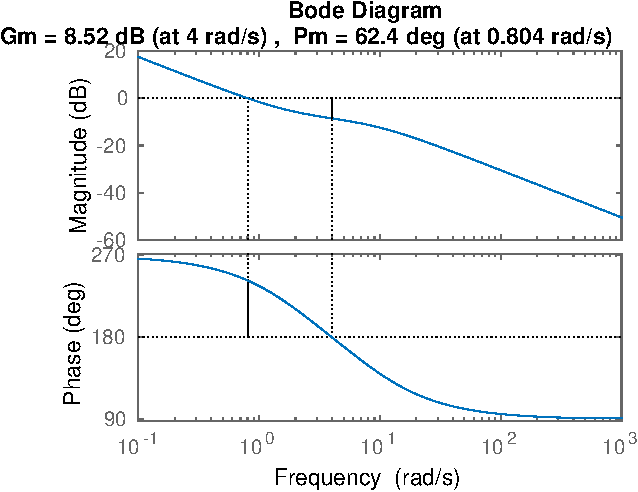
\includegraphics[width=0.5\linewidth]{bode-nonminopen-margin-crop}
  \end{center}

\textbf{(d)}
  Substitute
  \[ s' = \frac{2}{h}\frac{z-1}{z+1}\]
  in the transfer function for the controller this gives
  \[ F_d(z) = F(s')|_{s'=\frac{2}{h}\frac{z-1}{z+1}} = 3\frac{\frac{2}{h}\frac{z-1}{z+1}+2}{\frac{2}{h}\frac{z-1}{z+1} + 8} = 
3\frac{z-1 + h(z+1)}{z-1 + 4h(z+1)}\] 
\subsection{PID Tuning}
\label{sec-3-2}

   \textbf{(a)} The ultimate period is actually $T_u=\pi$:
     \begin{center}
     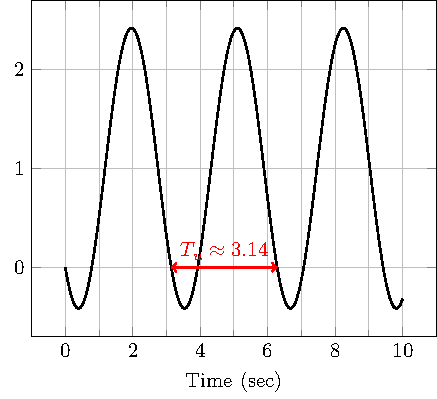
\includegraphics[width=0.5\linewidth]{bode-nonmincritical-solution}
     \end{center}

   \textbf{(b)} With $K_u=2$ and $T_u=\pi$, the Ziegler-Nicholls tuning is
   \[ F(s) = 1.2\left(1 + \frac{2}{\pi s} + \frac{\pi}{8} s \right) \]

   \textbf{(c)} Interesting differences between the two step responses:
\begin{itemize}
\item The tuned PID-controller has a rather high overshoot (more than 50\%). The controller from exercise 1 has no overshoot at all.
\item The tuned PID-controller has a short rise-time, but much longer settling time.
\item The tuned PID-controller gives a jump in the wrong direction at $t=0$. The other controller starts from zero, but starts off in the wrong direction.

     The open-loop transfer function with the tuned PID must have a much smaller phase margin (in fact the phase margin is $24.7\degree$ compared to $62.4\degree$). 

     The PID controlled system has an initial jump because there is a direct term from the input to the output. The open-loop system is given by
     \[ G_{o_{ZN}} = \frac{-0.47124 (s-2) (s+1.273)^2}{s^2 (s+2)} = -0.47124 + \frac{ 0.685s^2 + 1.636s + 1.527}{s^2 (s+2)} \]
     So at time $t=0$ the step in the command signal shows directly in $y$ multiplied with a negative factor. 

     The controller from exercise 1 gives a closed-loop system that starts in the wrong direction due to the right-hand side zero of $G(s)$. This can be seen by taking the derivative of the step-response and use the inital-value theorem. The derivative will be negative at time $t=0$. The derivative of the step response is simply the impulse response. Since the close loop system is given by
     \[ G_{c_{exc1}} = \left(\frac{-s+2}{s+2}\right)\frac{1}{1+s/3} \]
     the initial-value theorem gives
     \[ \lim_{t \to 0} \left(\frac{d}{dt} y_{step}(t)\right) = \lim_{t \to 0} y_{impulse}(t) = \lim_{s \to \infty} sG_{c_{exc1}}(s) = -\frac{1}{3}. \]

     \textbf{(d)} Backward difference gives the sampled controller 
     \begin{equation*}
       \begin{split}
        F_d(z) &= F_{ZN}(s')|_{s' = \frac{z-1}{zh}} =  1.2\left(1 + \frac{2}{\pi s} + \frac{pi}{8} s \right)|_{s' = \frac{z-1}{zh}}\\
               &= 1.2\left( 1 + \frac{2}{\pi \frac{z-1}{zh}} + \frac{\pi}{8} \frac{z-1}{zh}\right)
     \end{split}
     \end{equation*}
\end{itemize}

   

\end{document}
